\scanpage{166}
commutent aux p.d. --- et ils sont donnés par les couples $(\varphi_0,A'_1)$ satisfaisant 1) et 2) [on peut oublier 3)]. ; \deleted{cette condition tjrs vérifiée si $2$ est \unsure{inv.} dans $S'$} !

\uline{Corollaire 3} Pour que $\varphi_*$ respecte la filtration \inserted{(croiss. gross.)}, il f. et s. que
\[
 A'_1\in\operatorname{Fil}^{1}\quad\text{et}\quad B'_i\in\operatorname{Fil}^{i-1}\quad\forall i\geq1
\]
\[
 A'_1=\underbrace{a'_1}_{\lambda}X_0,\qquad
 B'_i=b'_{i0}+b'_{i1}X_0\mathbin{\text{---}}+b'_{i,i-1}X_0^{(i-1)}
 \qquad(a'_1,b'_{ij}\in S')
\]
[donc la condition 2) devient
\[
 (2')\quad a'_1t'=\varphi_0(t)
\]
et 3)
\[
 (3')\quad(2b'_{ij})J'=0\quad(i\geq1,\ 0\leq j\leq i-1)
\]
].

Pour que $\varphi_*$ respecte la \uline{graduation} \uline{et} les filtrations il f. et s. qu'on ait
\[
 A'_1=a'_1X_0,\qquad B'_i=0\quad i\geq0,
\]
alors, si de plus on suppose $S^+=(t)_{\mathrm{pd}}$, ces $\varphi$ correspondent exactt aux couples
\[
 (\varphi_0,\lambda):\deleted{\unsure{S\xrightarrow{\varphi_0}S'}}\inserted{(S,S^+,t)\mathbin{\text{---}}(S',S'^+,t')},
\]
par prolongement canonique :
\[
 \mathcal A_{S*}\mathbin{\text{---}}\mathcal A_{S'*}\ !
\]
\uline{Cor 4} $\varphi_*$ respecte \uuline{tjrs} la filtration \uline{décroissante}, associée aux degrés extérieurs.
\figure{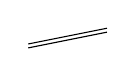
\begin{tikzpicture}\draw (0,0)--(1,.2);\draw (0,-.05)--(1,.15);\end{tikzpicture}}
Supposons maintenant
\[
 \begin{aligned}
 S&=k\{T\},&S^+&=(T)_{\mathrm{pd}},&t&=T\\
 S'&=k'\{T\},&S'^+&=(T)_{\mathrm{pd}},&t'&=T
 \end{aligned}
\]
\textcircled{1} La donnée de $\varphi_0$ correspond donc à la donnée de :
de \textcircled{a}
\[
 \varphi_{00}:k\mathbin{\text{---}}S'\deleted{\unsure{\{T\}}}=k'\{T\}
\]
(explicitable par un hom $k\xrightarrow{\delta_0}k'$ faisant de $k'$ un $k$-\unsure{module}) et des (\uline{op. diff.} $\delta_i$ $(i\geq1)$
\[
 \delta_i:k\mathbin{\text{---}}k'
\]
des tels que
\[
 \varphi_{00}(\lambda)=\sum_{i\geq0}\delta_i(\lambda)T^{(i)}
\]
On doit avoir
\[
 \begin{aligned}
 \delta_j(\unsure{1|u})&=0\quad j\geq1\\
 \delta_i(\lambda\lambda')&=\sum_{j+h=i}C_{j,h}\delta_j(\lambda)\delta_h(\lambda')\mathbin{\text{---}}
 \end{aligned}
\]
]
\margin{165}
